%%%%%%%%%%%%%%%%%%%%%%%%%%%%%%%%%%%%%%%%%
% University/School Laboratory Report
% LaTeX Template
% Version 3.1 (25/3/14)
%
% This template has been downloaded from:
% http://www.LaTeXTemplates.com
%
% Original author:
% Linux and Unix Users Group at Virginia Tech Wiki 
% (https://vtluug.org/wiki/Example_LaTeX_chem_lab_report)
%
% License:
% CC BY-NC-SA 3.0 (http://creativecommons.org/licenses/by-nc-sa/3.0/)
%
%%%%%%%%%%%%%%%%%%%%%%%%%%%%%%%%%%%%%%%%%

%----------------------------------------------------------------------------------------
%	PACKAGES AND DOCUMENT CONFIGURATIONS
%----------------------------------------------------------------------------------------

\documentclass{article}

\usepackage[version=3]{mhchem} % Package for chemical equation typesetting
\usepackage{siunitx} % Provides the \SI{}{} and \si{} command for typesetting SI units
\usepackage{graphicx} % Required for the inclusion of images
\usepackage{natbib} % Required to change bibliography style to APA
\usepackage{amsmath} % Required for some math elements 
\usepackage{hyperref} % Add link to text
\usepackage{comment} % Enable comment blocks

\setlength\parindent{0pt} % Removes all indentation from paragraphs

\renewcommand{\labelenumi}{\alph{enumi}.} % Make numbering in the enumerate environment by letter rather than number (e.g. section 6)

%\usepackage{times} % Uncomment to use the Times New Roman font

%----------------------------------------------------------------------------------------
%	DOCUMENT INFORMATION
%----------------------------------------------------------------------------------------

\title{Contract Scoping \\ With AADL and AGREE } % Title

\author{Danielle Stewart} % Author name

\date{April 2019} % Date for the report

\begin{document}

\maketitle % Insert the title, author and date

%\begin{center}
%\begin{tabular}{l r}
%Date Performed: & April, 2019 \\ % Date the experiment was performed
%Partners: & James Smith \\ % Partner names
%& Mary Smith \\
%Instructor: & Professor Heimdahl % Instructor/supervisor
%\end{tabular}
%\end{center}

% If you wish to include an abstract, uncomment the lines below
% \begin{abstract}
% Abstract text
% \end{abstract}

%----------------------------------------------------------------------------------------
%	SECTION 1
%----------------------------------------------------------------------------------------


%%%%%%%%%%%%%%%%%%%%%%%%%%%%%%%%%%%%%%%%%%%%%%%%%%%%
%				Problem Description
%%%%%%%%%%%%%%%%%%%%%%%%%%%%%%%%%%%%%%%%%%%%%%%%%%%%
\section{The Point of it All}

While working on the contracts and overall behavior of the large scale WBS, a problem rose regarding port names at various levels of the system (see Tech Report for more information about the WBS: \url{https://www.cs.umn.edu/sites/cs.umn.edu/files/tech_reports/18-007_0.pdf}). For instance, one of the top level inputs to the system is \textit{power}. This gets passed to lower level components and used in the contracts and is still called \textit{power}. To refer to this port value, the dot construction must be used (in both AADL and AGREE). One of the contracts in the BSCU refers to a few of these inputs that come from the top level and flow down. A direct child component of the BSCU (\textit{Channel}) has the same contract over its outputs/inputs as the BSCU, but the scope is different. 

While testing these contracts, it was seen that the lower level contract proves, but going up to the BSCU, the same contract does not prove. It was assumed that it is due to the scope of those ports - just because they have the same name does not mean they are the same value. This small system was created to illustrate the behavior of scoping in AADL and AGREE. It is located in the following repository: \url{https://github.com/dkstewart/University-Research/tree/master/Models} and is titled \textit{ContractScope}.

%%%%%%%%%%%%%%%%%%%%%%%%%%%%%%%%%%%%%%%%%%%%%%%%%%%%
%				Modes of Operation Description
%%%%%%%%%%%%%%%%%%%%%%%%%%%%%%%%%%%%%%%%%%%%%%%%%%%%
\section{Contract Scope Model Description}
The first version of the model has a top level component (\textit{Oberst}) and one child (\textit{Hauptmann}). The in and out ports are purposefully named the same thing in both levels. 

\begin{figure}[h]
\begin{center}
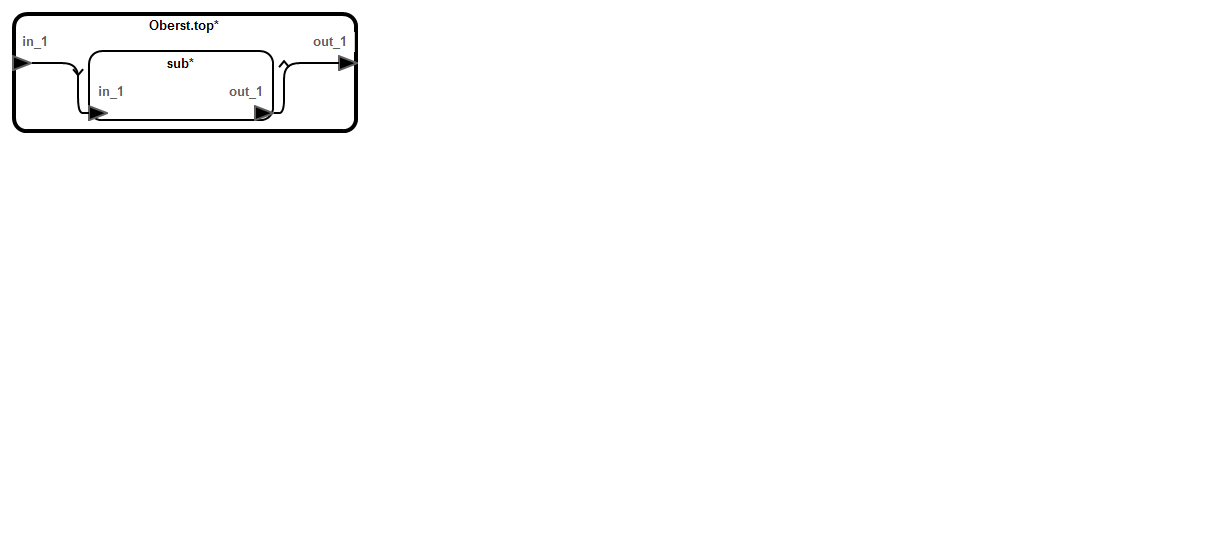
\includegraphics[width=300mm,scale=2.5]{images/good_connection} 
\vspace*{-105mm}
\caption{Structure of the Contract Scope system with connection}
\label{fig:connection}
\end{center}
\end{figure}

Top level component, \textit{Oberst}, has one boolean input (\textit{in\_1}) and one boolean output (\textit{out\_1}) . 

Subcomponents: 
\begin{itemize}
\item Hauptmann : One boolean input: \textit{in\_1} and one boolean output: \textit{out\_1}
\end{itemize}

The logic is very basic. In the child component, input equals output. There are no assumptions in the first version of the boolean model. 

\begin{figure}[h]
\begin{center}
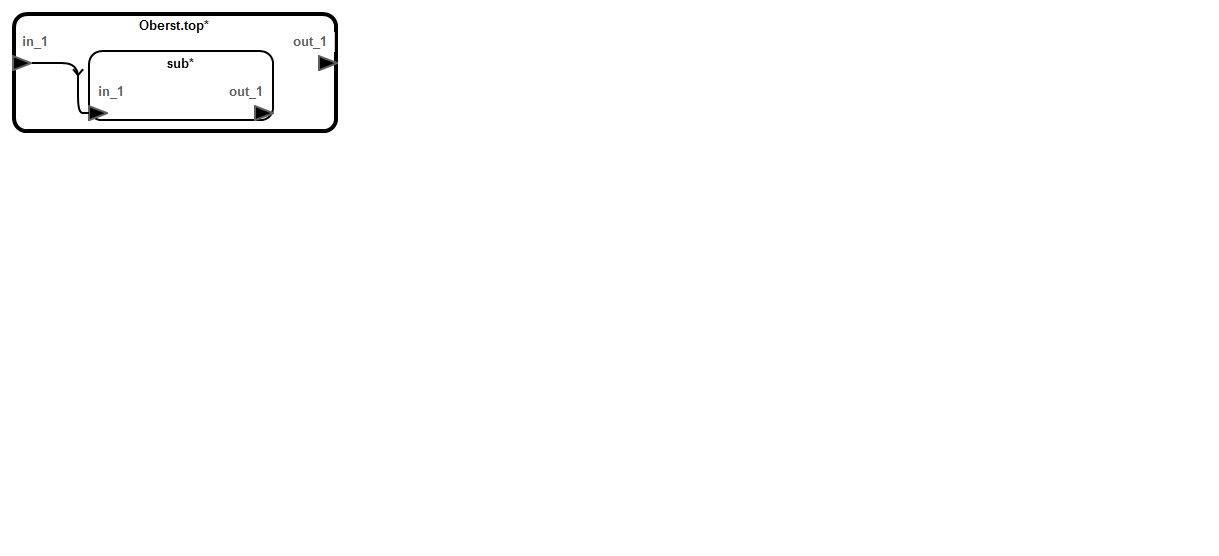
\includegraphics[width=300mm,scale=2.5]{images/broken_connection} 
\vspace*{-105mm}
\caption{Structure of the Contract Scope system without connection}
\label{fig:broken_connection}
\end{center}
\end{figure}

\section{Top Level Contracts and Testing}

There are a couple of main questions that we want to answer. \\

\textbf{1. If we lift up a property to a higher level and the ports are named the same, are we talking about different values/variables?}\\

To address this issue, I first just wrote a contract at the top level stating that output at the top equals output of the subcomponent. \\

\textit{``Top level output equals sub level output.''}\\
$out\_1 = sub.out\_1$\\

We expect this to be true AS LONG AS the connection port is defined between the child component output and the top level output (see Figure~\ref{fig:connection}. When running the analysis with the connection in place, this proves. If the connection between these ports is commented out (Figure~\ref{fig:broken_connection}), this lemma fails to prove. If the input connection is severed, this lemma still proves. The output is all that matters.\\

Likewise, I wrote a contract stating that the top level input equals the top level output.\\
$in\_1 = out\_1$\\

The only contract that guarantees that this should be true is in the child component. Therefore if all connections are sound, this proves. Of course, if not, it does not prove. This is true for both the input and output connections.\\

\begin{figure}[h]
\begin{center}
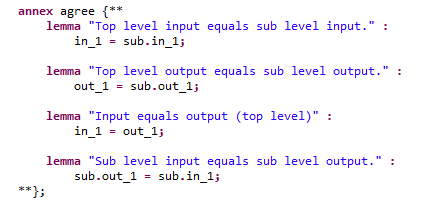
\includegraphics[width=1.2\textwidth]{images/lemmas} 
\caption{Top level contracts for boolean model}
\label{fig:lemmas}
\end{center}
\end{figure}

All top level contracts are shown in Figure~\ref{fig:lemmas}. \\

\textbf{2. What is the initial state of the system? Do we need to wait a step before the top level output port reflects the contract of the child component?}\\

To answer this question and really see initial behavior as well as test the contracts using the ``$\rightarrow$'' operator, a second version of the system was made. The components and connections are the same, but the ports are integers and there are new assumptions. These integers are bounded between 0 and 10 and the initial value of the input is 1. See Figure~\ref{fig:assume}.\\

\begin{figure}[h]
\begin{center}
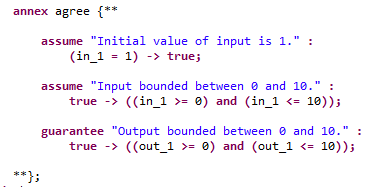
\includegraphics[width=0.95\textwidth]{images/toplevelassumptions} 
\caption{Top level assumptions for integer model}
\label{fig:assume}
\end{center}
\end{figure}

The first round, I left in all the lemmas as shown in Figure~\ref{fig:lemmas} and added the ``$\rightarrow$' operator. All prove with connections declared. No ``prev''  operators are required anywhere in the model.\\

When running the analysis with the connection in place, this proves. If the connection between these ports is commented out (Figure~\ref{fig:broken_connection}), this lemma fails to prove. All top level contracts are shown in Figure~\ref{fig:lemmas}. 

As a further test (mostly out of curiousity), I took out the ``$\rightarrow$'' operator from the top level lemmas. Partly this is to check behavior when it is removed and partly to see whether we need consistency regarding this operator and if so, why. 

The results of verification are shown in Figure~\ref{fig:failed1}. 
\begin{figure}[h]
\begin{center}
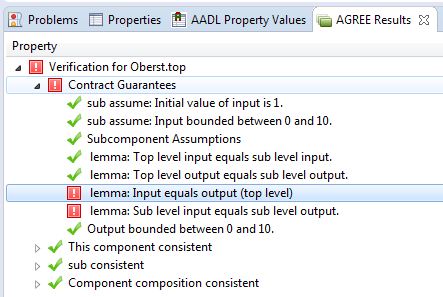
\includegraphics[width=0.75\textwidth]{images/failed1} 
\caption{Verification for integer model without use of arrow operator}
\label{fig:failed1}
\end{center}
\end{figure}

The counterexamples existed in the initial state of the system and showed for both of these failed contracts that when we do not specify initial state in the top level properties, the inputs follow the assumptions (equal to 1), but the output is unconstrained. See Figures~\ref{fig:coex1} and ~\ref{fig:coex2}.
\begin{figure}[h]
\begin{center}
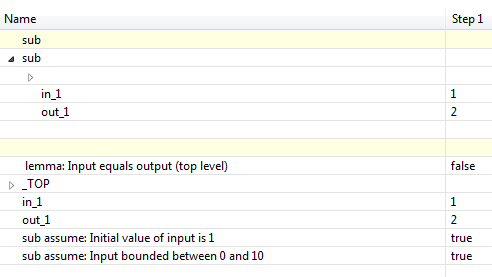
\includegraphics[width=0.75\textwidth]{images/coex1} 
\caption{Counterexample for top level input equals top level output}
\label{fig:coex1}
\end{center}
\end{figure}

\begin{figure}[h]
\begin{center}
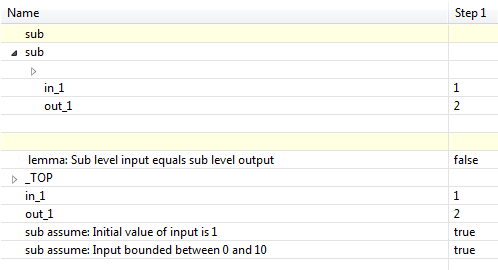
\includegraphics[width=0.75\textwidth]{images/coex2} 
\caption{Counterexample for sub level input equals sub level output}
\label{fig:coex2}
\end{center}
\end{figure}

I then changed the subcomponent contract regarding the output to \textit{exclude} the arrow operator. Thus the guarantee was then simply: \\
\begin{figure}[h]
\begin{center}
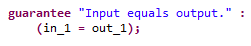
\includegraphics[width=0.75\textwidth]{images/output_contract} 
\caption{Countract on output without arrow operator}
\label{fig:output_contract}
\end{center}
\end{figure}

With this in place, all lemmas prove at the top level. \\

Thus when using the arrow operator and defining a particular initial state, any behavior that should hold in ALL states should not have the arrow operator. It is not required to be consistent through the model, just correctly define the inital state. If it is not important what the behavior of a component is in the initial state, then we can use ``true $\rightarrow$''. If it is important, it is sufficient to eliminate that operator. This causes the guarantee to apply in all states.


\section{Thoughts}

Scoping is pretty clear. As long as the connections are in place, the scope is what we thought it was. If the connections are nonexistant in the model, then the scope and behavior of component in scope determines proof of contract in question. \\

Of course initial behavior adds some complexity to the behavior model, but one thing that seems important is this: Our top level lemmas should prove in every state including initial state. If we add initial state behavior to a model through the arrow operator, it might be prudent to keep the arrow operator out of the top level contracts. This forces us to implement correct initial behavior in all of the pertinant subcomponents whose contracts are used in the proof of the top level properties.

















% If you have more than one objective, uncomment the below:
%\begin{description}
%\item[First Objective] \hfill \\
%Objective 1 text
%\item[Second Objective] \hfill \\
%Objective 2 text
%\end{description}

%\subsection{Definitions}
%\label{definitions}
%\begin{description}
%\item[Stoichiometry]
%The relationship between the relative quantities of substances taking part in a reaction or forming a compound, typically a ratio of whole integers.
%\item[Atomic mass]
%The mass of an atom of a chemical element expressed in atomic mass units. It is approximately equivalent to the number of protons and neutrons in the atom (the mass number) or to the average number allowing for the relative abundances of different isotopes. 
%\end{description} 
 
 \begin{comment}
 
%----------------------------------------------------------------------------------------
%	SECTION 2
%----------------------------------------------------------------------------------------

\section{Experimental Data}

\begin{tabular}{ll}
Mass of empty crucible & \SI{7.28}{\gram}\\
Mass of crucible and magnesium before heating & \SI{8.59}{\gram}\\
Mass of crucible and magnesium oxide after heating & \SI{9.46}{\gram}\\
Balance used & \#4\\
Magnesium from sample bottle & \#1
\end{tabular}

%----------------------------------------------------------------------------------------
%	SECTION 3
%----------------------------------------------------------------------------------------

\section{Sample Calculation}

\begin{tabular}{ll}
Mass of magnesium metal & = \SI{8.59}{\gram} - \SI{7.28}{\gram}\\
& = \SI{1.31}{\gram}\\
Mass of magnesium oxide & = \SI{9.46}{\gram} - \SI{7.28}{\gram}\\
& = \SI{2.18}{\gram}\\
Mass of oxygen & = \SI{2.18}{\gram} - \SI{1.31}{\gram}\\
& = \SI{0.87}{\gram}
\end{tabular}

Because of this reaction, the required ratio is the atomic weight of magnesium: \SI{16.00}{\gram} of oxygen as experimental mass of Mg: experimental mass of oxygen or $\frac{x}{1.31}=\frac{16}{0.87}$ from which, $M_{\ce{Mg}} = 16.00 \times \frac{1.31}{0.87} = 24.1 = \SI{24}{\gram\per\mole}$ (to two significant figures).

%----------------------------------------------------------------------------------------
%	SECTION 4
%----------------------------------------------------------------------------------------

\section{Results and Conclusions}

The atomic weight of magnesium is concluded to be \SI{24}{\gram\per\mol}, as determined by the stoichiometry of its chemical combination with oxygen. This result is in agreement with the accepted value.

%\begin{figure}[h]
%\begin{center}
%
\includegraphics[width=0.65\textwidth]{placeholder} % Include the image placeholder.png
%\caption{Figure caption.}
%\end{center}
%\end{figure}

%----------------------------------------------------------------------------------------
%	SECTION 5
%----------------------------------------------------------------------------------------

\section{Discussion of Experimental Uncertainty}

The accepted value (periodic table) is \SI{24.3}{\gram\per\mole} \cite{Smith:2012qr}. The percentage discrepancy between the accepted value and the result obtained here is 1.3\%. Because only a single measurement was made, it is not possible to calculate an estimated standard deviation.

The most obvious source of experimental uncertainty is the limited precision of the balance. Other potential sources of experimental uncertainty are: the reaction might not be complete; if not enough time was allowed for total oxidation, less than complete oxidation of the magnesium might have, in part, reacted with nitrogen in the air (incorrect reaction); the magnesium oxide might have absorbed water from the air, and thus weigh ``too much." Because the result obtained is close to the accepted value it is possible that some of these experimental uncertainties have fortuitously cancelled one another.

%----------------------------------------------------------------------------------------
%	SECTION 6
%----------------------------------------------------------------------------------------

\section{Answers to Definitions}

\begin{enumerate}
\begin{item}
The \emph{atomic weight of an element} is the relative weight of one of its atoms compared to C-12 with a weight of 12.0000000$\ldots$, hydrogen with a weight of 1.008, to oxygen with a weight of 16.00. Atomic weight is also the average weight of all the atoms of that element as they occur in nature.
\end{item}
\begin{item}
The \emph{units of atomic weight} are two-fold, with an identical numerical value. They are g/mole of atoms (or just g/mol) or amu/atom.
\end{item}
\begin{item}
\emph{Percentage discrepancy} between an accepted (literature) value and an experimental value is
\begin{equation*}
\frac{\mathrm{experimental\;result} - \mathrm{accepted\;result}}{\mathrm{accepted\;result}}
\end{equation*}
\end{item}
\end{enumerate}

%----------------------------------------------------------------------------------------
%	BIBLIOGRAPHY
%----------------------------------------------------------------------------------------

\bibliographystyle{apalike}

\bibliography{biblio}

%----------------------------------------------------------------------------------------
\end{comment}

\end{document}